\section{Analyzing Algorithms}

\emph{Asymptotic analysis}, or in general, the analysis of function growth, relates heavily to the performance of an algorithm. 
We can represent algorithms as mathematical functions and describe their relative performance in terms of the input size. 

\myexample{Consider the linear search algorithm.} 
We know that, in the best case, the item that we are searching for is the first element in the list. 
In the average case, it is found in the middle of the list. In the worst case, the element does not exist in the list. 
Because we have to traverse through~$n$ elements, namely the~$n$ elements of our input list, we say that the linear search grows linearly in proportion to its input size. \emph{Best-case}\index{best case}, \emph{average-case}\index{average case}, and \emph{worst-case}\index{worst case} describe the potential inputs to a function. 
We can ascribe similar attributes to binary search, the sorting algorithms from the previous chapter and beyond. 
Though, we need a notation to denote the growth rate of a function. 
In computer science, we most often make use of \emph{Big-Oh notation}\index{Big-Oh notation}\index{Big-Oh}, which denotes the upper bound on the growth of a function. 
That is, a function $f(n) = \mathcal{O}(g(n))$ if, at some point,~$f(n)$ begins to forever grow slower than or equal to~$g(n)$. 
We can roughly replace the equals~`$=$' sign with a less-than-or-equal-to~`$\leq$' sign. 
One detail to note is that the end-behavior of a polynomial is determined by its highest-order term. 
For example, $f(n) = 0.5x^2 + 0.5\cos(\textsf{deg}(5x))$ is upper-bounded by $g(n) = 0.5x^2$, because the cosine function is upper-bounded by~$1$. 
When describing a function in terms of asymptotic bounds, we can drop/ignore all coefficients and lower-order terms.

\myexample{Consider the following functions $f(n) = 0.5x^2 + 0.5\cos(\textsf{deg}(5x))$ and $g(n) = 0.2x^3 + 0.3\sin({\textsf{deg}(4x)})$.} 
As we stated, we can drop all lower-order terms and coefficients, meaning $f(n) = n^2$ and $g(n) = n^3$. 
From here, it is trivial to see that for any $n \geq 1$, $g(n)$ grows faster (or at least as fast) than $f(n)$.
Thus, we say that $f(n) = \mathcal{O}(g(n))$.\footnote{There is a bit more to the formalism of Big-Oh, but we will explain those details in due time.}

\begin{figure}[H]
  \centering
  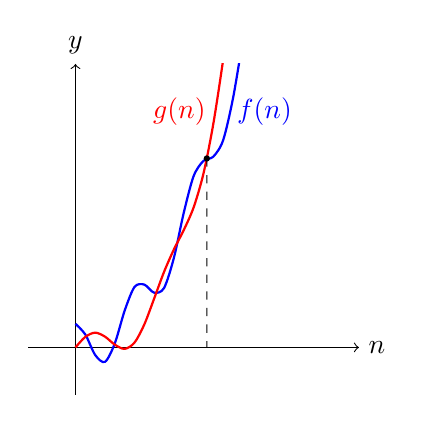
\begin{tikzpicture}[scale=0.6]
      % Axes
      \draw[->] (-1,0) -- (6,0) node[right] {$n$};
      \draw[->] (0,-1) -- (0,6) node[above] {$y$};
  
      \begin{scope}
      \clip (-1,-1) rectangle (5,6);
      % Function g(n)
      \draw[domain=0:5, smooth, thick, blue] plot (\x, {0.5*\x^2 + 0.5*cos(deg(5*\x))});
      \node[blue] at (4,5) {$f(n)$};
      
      % Function f(n)
      \draw[domain=0:5, smooth, thick, red] plot (\x, {0.2*\x^3 + 0.3*sin(deg(4*\x))});
      \node[red] at (2.2,5) {$g(n)$};
      \end{scope}
      % Big-Oh notation
      \coordinate (intersection) at (2.78, 4.0);
      \fill[black] (intersection) circle (1.9pt);
      \draw[dashed] (intersection) -- (2.78,0);
  \end{tikzpicture}
  \caption{$f(n) = \mathcal{O}(g(n))$}
  \end{figure}

There are two other common notations for asymptotic analysis: Big-Omega and Theta. 
\emph{Big-Omega}\index{Big-Omega notation}\index{Big-Omega} describes the lower-bound of the growth of a function, and Theta\index{Theta notation}\index{Theta} describes the tight bound of a function. 
That is, $f(n) = \Omega(g(n))$ if there is a point at which $f(n)$ begins to grow faster than or equal to $g(n)$. 
We can roughly replace the equals `$=$' sign with a greater-than-or-equal-to `$\geq$' relation. 
Similarly, $f(n) = \Theta(g(n))$ if $f(n) = \mathcal{O}(g(n))$ and $f(n) = \Omega(g(n))$. 
We can roughly replace the equals `$=$' sign with an equivalence `$\equiv$' sign. 
Examples for Omega and Theta are harder to come by without a formalized definition, so we will defer them until later.

\begin{figure}[H]
  \centering
  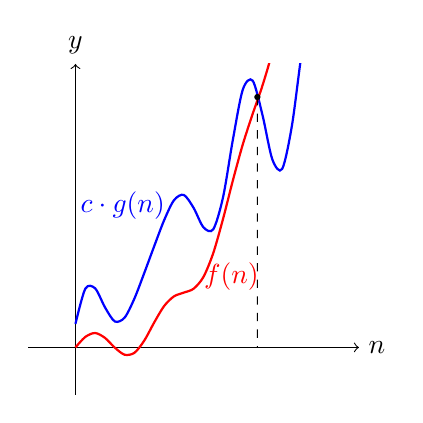
\begin{tikzpicture}[scale=0.6]
    % Axes
    \draw[->] (-1,0) -- (6,0) node[right] {$n$};
    \draw[->] (0,-1) -- (0,6) node[above] {$y$};

    \begin{scope}
    \clip (-1,-1) rectangle (5,6);
    % Function g(n)
    \draw[domain=0:5, smooth, thick, blue] plot (\x, {1.2*\x + 0.5*cos(deg(5*\x)) + sin(deg(4*\x))});
    \node[blue] at (1,3) {$c\cdot{}g(n)$};
    
    % Function f(n)
    \draw[domain=0:5, smooth, thick, red] plot (\x, {0.09*\x^3 + 0.3*sin(deg(4*\x))});
    \node[red] at (3.3, 1.5) {$f(n)$};
    \end{scope}
    % Big-Oh notation
    \coordinate (intersection) at (3.85, 5.3);
    \fill[black] (intersection) circle (1.9pt);
    \draw[dashed] (intersection) -- (3.85,0);
\end{tikzpicture}
\caption{$f(n) = \Omega(g(n))$}
\end{figure}

\begin{figure}[H]
  \centering
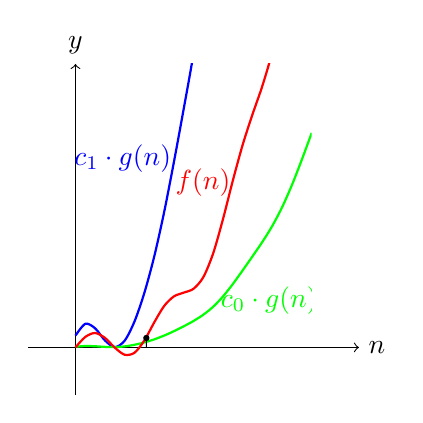
\begin{tikzpicture}[scale=0.6]
  % Axes
  \draw[->] (-1,0) -- (6,0) node[right] {$n$};
  \draw[->] (0,-1) -- (0,6) node[above] {$y$};

  \begin{scope}
  \clip (-1,-1) rectangle (5,6);
  % Function g(n)
  \draw[domain=0:5, smooth, thick, blue] plot (\x, {0.5*(0.8*\x^3 + 0.5*cos(deg(5*\x)) + sin(deg(4*\x))});
  \node[blue] at (1,4) {$c_1\cdot{}g(n)$};

  \draw[domain=0:5, smooth, thick, green] plot (\x, {0.03*(1.2*\x^3 + 0.5*cos(deg(5*\x)) + sin(deg(4*\x))});
  \node[green] at (4.1,1) {$c_0\cdot{}g(n)$};
  
  % Function f(n)
  \draw[domain=0:5, smooth, thick, red] plot (\x, {0.09*\x^3 + 0.3*sin(deg(4*\x))});
  \node[red] at (2.7, 3.5) {$f(n)$};
  \end{scope}
  % Big-Oh notation
  \coordinate (intersection) at (1.5, 0.2);
  \fill[black] (intersection) circle (1.9pt);
  \draw[solid] (intersection) -- (1.5,0);
\end{tikzpicture}
\caption{$f(n) = \Theta(g(n))$}
\end{figure}

The term ``asymptotic analysis'' stems from the fact that ``asymptotic'' behavior describes the behavior of a function as its input approaches infinity. 

Programmers often conflate Big-Oh as meaning the ``worst-case'' of an algorithm, Big-Omega as the ``best case,'' and Theta as the ``average case.'' 
In actuality, these have no precise and deterministic relation to one another, and this misconception will be further addressed in a subsequent section. 
Remember that Big-Oh is the upper-bound, Big-Omega is the lower-bound, and Theta exists if the function is Big-Oh and Big-Omega of the same function.

\myexample{Consider the following function.}
\begin{verbnobox}[\small]
// foo receives an array of integers.
foo(ls) {
  // v is a random integer between 0 and 100, with equal probability.
  v := RNG()
  n := len(ls)
  if v == 100
    return 42
  else if v == 0
    for i := 0 to n do
      for j := 0 to n do
        n := n + i * j;
  else
    for i := 0 to n do
      n := n + i;
  return n;
}
\end{verbnobox}

The best-case for this algorithm is for~$v$ to be~$100$, meaning we immediately return~$42$. 
Therefore, we are upper-bounded by~$\mathcal{O}(1)$, since this is a constant-time operation. 
We are similarly lower-bounded by this operation, meaning it is~$\Omega{(1)}$. 
Therefore, it is also~$\Theta(1)$ in the best case.

In the worst case,~$v$ is zero, meaning we have a nested for-loop over the length of the input list, meaning we are (strictly) upper-bounded by~$\mathcal{O}(n^2)$. 
The \ttt{for}-loops must always execute, meaning that we are lower-bounded by~$\Omega(n^2)$ as well. 
We can conclude similar reasoning for~$\Theta(n^2)$.

In the average case, i.e., when~$n$ is neither~$0$ nor~$100$, we loop once over the length of the input list, meaning we are both upper and lower-bounded by~$\mathcal{O}(n)$ and~$\Omega(n)$ respectively.

\myexample{Recall the binary search algorithm.} 
In the best case, we find the element immediately. 
Therefore, we can conclude that we are lower-bounded by~$\Omega(1)$, but we can also reasonably conclude that we are upper-bounded by~$\mathcal{O}(n^3)$. 
This reasoning seems odd, but it's certainly true; finding the element immediately will never exceed~$\mathcal{O}(n^3)$. 
It's logically correct to conclude that we are upper-bounded by~$\mathcal{O}(n^n)$ as well; we will never grow faster than~$\mathcal{O}(n^n)$. 
These are what we call \emph{loose (upper)-bounds}, and are a bit sloppy to state for binary search. 
In the best case, we find the element immediately, so proclaiming anything other than that the upper-bound is~$\mathcal{O}(1)$ is, while technically correct, loose. 
Moreover, in these instances, should we say that the upper-bound is not~$\mathcal{O}(1)$ in the best case, we lose the ability to conclude that the algorithm, in the best case, is~$\Theta(1)$.

In the worst case, the element is not in the list. 
Therefore, we are upper-bounded by~$\mathcal{O}(\lg{n})$, but lower-bounded, yet again, by~$\Omega(\lg\lg{n})$. 
This is similarly a sloppy argument to make, because while it is true that we will never find the element faster that~$\Omega(\lg\lg{n})$ in the worst case, it's not a tight lower bound, meaning we lose the ability to use Theta notation, should we opt for this lower bound.

In the average case, we land somewhere in the middle of finding the element immediately and it not existing at all, meaning that we are upper-bounded by~$\mathcal{O}(\lg{n})$, and lower-bounded bounded by~$\Omega(1)$. 
Therefore, concluding~$\Theta(\lg{n})$ is incorrect for binary search.

\myexample{Recall the insertion sort algorithm.} 
We can analyze that, in the best case, the structure is already sorted, meaning nothing needs to be (recursively) sorted and inserted. 
Therefore, we require exactly one traversal over the data, meaning it is upper-bounded by~$\mathcal{O}(n)$. 
Additionally, because we do require exactly one traversal over the input data, we are also lower-bounded by~$\Omega(n)$. 
Hence, we can also conclude that, in the best-case, insertion sort is~$\Theta(n)$.

In the worst-case, the list is in reversed order. 
So, we must insert each element in the correct position, with respect to every other element. 
Therefore we are upper and lower-bounded by~$\mathcal{O}(n^2)$ and~$\Omega(n^2)$ respectively.

\subsection{Formalizing Big-Oh, Big-Omega, and Theta}
We have informally introduced Big-Oh, Big-Omega, and Theta notations. 
For proving a mathematical function's asymptotic bounds, a formal demonstration is essential. 
In the following subsections, we will outline these important demonstrations.

\subsubsection*{Big-Oh}
A function $f(n) = \mathcal{O}(g(n))$ if there exists a constant~$c > 0$ and a number~$n_0$ such that $f(n) \leq cg(n)$ for every~$n \geq n_0$~\Citep{clrs}. 
Interestingly, we can describe all three notations in terms of limits. 
We say that $f(n) = \mathcal{O}(g(n))$ if $\lim_{n \to \infty} \frac{f(n)}{g(n)} < \infty$. 
Unfortunately there is no hard-and-fast rule to apply when finding the~$c$ and~$n_0$ constants. 
What is convenient about it, however, is that multiple solutions may work, hence the existential quantifiers in the definition.

\myexample{Prove that $3n^2 + 6n = \mathcal{O}(n^2)$.} 
We need to find a constant~$c > 0$ and a number~$n_0$ such that~$3n^2 + 6n \leq cn^2$ for every~$n \geq n_0$. 
Let's move~$3n^2$ to the right-hand side of the inequality and divide both sides by~$n^2$.

\begin{align*}
  3n^2 + 6n &\leq cn^2\\
  6n &\leq cn^2 - 3n^2\\
  6n &\leq n^2(c - 3)\\
  \frac{6n}{n^2} &\leq c - 3\\
  \frac{6}{n} &\leq c - 3\\
  \frac{6}{n} + 3 &\leq c\\
  c &\geq \frac{6}{n} + 3
\end{align*}

If we assign~$n$ to be~$1$, then~$c \geq 9$, and the inequality holds for all~$n \geq 1$. Therefore we can conclude that~$3n^2 + 6n = \mathcal{O}(n^2)$. We can also evaluate this as a limit:

\begin{align*}
  \lim_{n \to \infty} \frac{3n^2 + 6n}{n^2} &= \lim_{n \to \infty} \frac{3n^2}{n^2} + \frac{6n}{n^2}\\
  &= \lim_{n \to \infty} 3 + \frac{6}{n}\\
  &= 3 + 0\\
  &= 3 < \infty
\end{align*}

\myexample{Prove that $0.25n^4 - 6000n^3 + 25 \neq \mathcal{O}(n^3)$.} 
To show that this relationship does not hold, we can do either a proof-by-contradiction or use the limit definition. 
Let's write a proof-by-contradiction. 
Assume the opposite, that $0.25n^4 - 6000n^3 + 25 = \mathcal{O}(n^3)$. 
Then there exists a constant~$c > 0$ and a number~$n_0$ such that $0.25n^4 - 6000n^3 + 25 \leq cn^3$ for every~$n \geq n_0$.

\begin{align*}
  0.25n^4 - 6000n^3 + 25 &\leq cn^3\\
  25 &\leq cn^3 - 0.25n^4 + 6000n^3\\
  25 &\leq n^3(c + 0.25n + 6000)\\
  \frac{25}{n^3} &\leq c + 0.25n + 6000\\
  c &\geq \frac{25}{n^3} - 0.25n - 6000
\end{align*}

The problem here is that, no matter what constant we choose for~$c$, there is always an~$n\in\mathbb{N}$ that falsifies the inequality. 
Therefore we can conclude that $0.25n^4 - 6000n^3 + 25 \neq \mathcal{O}(n^3)$. 
We can also evaluate this as a limit:

\begin{align*}
  \lim_{n \to \infty} \frac{0.25n^4 - 6000n^3 + 25}{n^3} &= \lim_{n \to \infty} \frac{0.25n^4}{n^3} - \frac{6000n^3}{n^3} + \frac{25}{n^3}\\
  &= \lim_{n \to \infty} 0.25n - 6000 + \frac{25}{n^3}\\
  &= \infty - 6000 + 0\\
  &= \infty
\end{align*}

\myexample{Prove that $(2n^2 + n)(4n) = \mathcal{O}(n^3)$.} 
Expanding the expression, we get~$8n^3 + 4n^2$, meaning we need to find constants~$c$ and~$n_0$ such that $8n^3 + 4n^2 \leq cn^3$ for all $n\geq n_0$.

\begin{align*}
  8n^3 + 4n^2 &\leq cn^3\\
  4n^2 &\leq cn^3 - 8n^3\\
  4n^2 &\leq n^3(c - 8)\\
  \frac{4n^2}{n^3} &\leq c - 8\\
  \frac{4}{n} &\leq c - 8\\
  \frac{4}{n} + 8 &\leq c\\
  c &\geq \frac{4}{n} + 8
\end{align*}

For~$n_0=1$, we have~$c\geq 12$. 
Therefore we can conclude that $(2n^2 + n)(4n) = \mathcal{O}(n^3)$. 
We can also evaluate this as a limit:

\begin{align*}
  \lim_{n \to \infty} \frac{(2n^2 + n)(4n)}{n^3} &= \lim_{n \to \infty} \frac{8n^3 + 4n^2}{n^3}\\
  &= \lim_{n \to \infty} 8 + \frac{4}{n}\\
  &= 8 + 0\\
  &= 8 < \infty
\end{align*}

\myexample{Prove that $(4n)^n \neq \mathcal{O}(n^n)$.} 
Assume the opposite, $(4n)^n = \mathcal{O}(n^n)$. 
Then, there exists a constant~$c > 0$ and a number~$n_0$ such that $(4n)^n \leq cn^n$ for every~$n \geq n_0$. 
Expanding the left-hand side, then dividing both sides by~$n^n$ gets us:

\begin{align*}
  4^n \cdot n^n &\leq cn^n\\
  4^n &\leq c
\end{align*}

The problem is that we cannot pick a constant~$c$ without finding an~$n$ that falsifies the inequality. 
Therefore, by contradiction, $(4n)^n \neq \mathcal{O}(n^n)$.

\myexample{Prove that $3n + n\lg{n} = \mathcal{O}(n^2)$.} 
Dividing both sides of the equation by~$n$ gets us:

\begin{align*}
  3n + n\lg{n} &\leq cn^2\\
  3 + \lg{n} &\leq cn\\
  \lg{n} \leq cn - 3
\end{align*}

Suppose~$c = 3$. 
Then,~$\lg{n} \leq n$ for any~$n > 2$, so we can let $n_0 = 3$. 
Thus, $3n + n\lg{n} = \mathcal{O}(n^2)$.

\subsubsection*{Big-Omega}
A function $f(n) = \Omega(g(n))$ if there exists a constant~$c > 0$ and a number~$n_0$ such that $f(n) \geq cg(n)$ for every $n \geq n_0$. 
We can describe this in terms of limits as well. 
We say that $f(n) = \Omega(g(n))$ if $\lim_{n \to \infty} \frac{f(n)}{g(n)} > 0$.

\myexample{Prove that $(2n^3 - 6n^2) = \Omega(n^2)$.} 
We need to find a constant~$c > 0$ and a number~$n_0$ such that $(2n^3 - 6n^2) \geq cn^2$ for every $n \geq n_0$. 
First, let's factor out the~$n^2$ on the left-hand side of the inequality.

\begin{align*}
  2n^3 - 6n^2 &\geq cn^2\\
  n^2(2n - 6) &\geq cn^2\\
  2n - 6 &\geq c\\
  c &\leq 2n - 6\\
\end{align*}

We know that~$2n - 6$ is always greater than $0$ for~$n > 3$, so we will let~$n_0 = 4$ and~$c_0 = 1$. 
Therefore, we can conclude that $(2n^3 - 6n^2) = \Omega(n^2)$.

\myexample{Prove that $3n^2 + 4n - 8 = \Omega(n^2)$.} 
We need to find a constant~$c > 0$ and a number~$n_0$ such that $3n^2 + 4n - 8 \geq cn^2$ for every $n \geq n_0$.
We can divide both sides by~$n^2$:

\begin{align*}
  3n^2 + 4n - 8 &\geq cn^2\\
  3 + \frac{4}{n} - \frac{8}{n^2} &\geq c\\
  c &\leq 3 + \frac{4}{n} - \frac{8}{n^2}
\end{align*}

Choosing~$n_0 = 8$, we need a value of~$c$ to satisfy the inequality $c \leq 3 + \frac{1}{2} - \frac{1}{64}$, which reduces to $c \leq 3.484375$. 
So, picking~$c = 3$ works, and we have proved that $3n^2 + 4n - 8 = \Omega(n^2)$.

\subsubsection*{Theta}
A function $f(n) = \Theta(g(n))$ if there exists constants~$c_0, c_1 > 0$ and a point~$n_0$ such that $c_0g(n) \leq f(n) \leq c_1g(n)$ for every $n \geq n_0$. 
We can also say that $f(n) = \Theta(g(n))$ if $f(n) = \mathcal{O}(g(n))$ and $f(n) = \Omega(g(n))$.

\subsection{Misconceptions About Asymptotic Analyses}

As we mentioned before, many programmers conflate best, average, and worst-cases with Big-Omega, Theta, and Big-Oh respectively. \emph{There is no discernible relationship between these concepts.}

\myexample{Consider the absolutely egregious statement, ``linear search is $n$.''} 
The big problem here is that we are using~$n$ without any qualification;~$n$ what? 
A slightly better, but still poor, way to phrase it is, ``linear search is $\mathcal{O}(n)$,'' which introduces the upper-bound. 
The problem now is that we have yet to state under what conditions is linear search~$\mathcal{O}(n)$, i.e., best-case, average-case, or worst-case. 
So, we can state, ``linear search, in the worst-case, is $\mathcal{O}(n)$.'' 
Even though this is an accurate statement, using a loose upper-bound when the lower-bound is known and is equal to the upper-bound is sloppy. 
We \emph{should} assert that, ``linear search, in the worst-case, is $\Theta(n)$,'' which is a tight bound. 
Being specific about the conditions under which an algorithm is $\mathcal{O}(n)$, $\Omega(n)$, or $\Theta(n)$ is important, as is using tightened bounds when possible.

\myexample{Consider the statement, ``Insertion sort is faster than merge sort since it is $\mathcal{O}(n)$ while merge sort is $\Theta(n\lg{n})$.''\footnote{Thanks, Steve Tate, for this (practice) exam problem.}} 
There are two problems with such a claim: first, it omits the qualification of what case analysis we wish to reference. 
To fix it, we need to add ``in the best case'' immediately after ``is faster than merge sort.'' 
Second, we could tighten the bound of insertion sort because it is~$\mathcal{O}(n)$ and $\Omega(n)$ in the best case.

\myexample{Consider the statement, ``The worst-case running time of selection sort is $\mathcal{O}(n^2)$ and the worst-case running time of merge sort is $\mathcal{O}(n\lg{n})$; therefore, merge sort is asymptotically faster in the worst-case.''} 
Is this statement correct? 
Unfortunately, it is not, and we can fix the statement by changing only the asymptotic functions. 
It is incorrect because Big-Oh only describes the upper-bound of a function. 
We cannot conclude that merge sort is asymptotically faster in the worst-case because we do not know the lower-bound of either algorithm. 
To correct the statement, we ascribe a tight-bound on the growth of the functions via $\Theta(n^2)$ and $\Theta(n\lg{n})$ respectively. 
We could also just place the tight-bound on only $\Theta(n^2)$, which then provides the lower-bound of selection sort, but as we have continuously stated, using tight-bounds is always the preferred option.

\subsection{Analysis of the Sorting Algorithms}

We can analyze the five sorting algorithms described in Chapter~\ref{chapter-searching-sorting} in terms of their asymptotic behavior in the best, average, and worst cases.

\subsubsection*{Bubble Sort}
Starting off with bubble sort, in the best case, the array is already sorted, meaning we only need to traverse the array once. 
Therefore, we are upper and lower-bounded by~$\mathcal{O}(n)$ and~$\Omega(n)$ respectively. 
Hence, we can conclude that bubble sort is~$\Theta(n)$ in the best case. 

In the average case, each element is roughly ``half way'' to its sorted position. 
We can compute the expected number of swaps/inversions as follows: an array of length~$n$ has an inversion~$I_{i, j} = 1$ if we must swap the values~$(i, j)$. 
Therefore, the expected value of there being an inversion for any arbitrary pair is~$1/2$ because either a pair must or must not be inverted. 
Our loop traverses from~$i=1$ to~$n$, with an inner loop of~$j>i$ to~$n$. 
In the average case, each element is roughly ``half way'' to its sorted position. 
We can compute the expected number of swaps/inversions as follows: an array of length~$n$ has an inversion~$I_{i, j} = 1$ if we must swap the values~$(i, j)$. 
Therefore, the expected value of there being an inversion for any arbitrary pair is~$1/2$ because either a pair must or must not be inverted. 
Our loop traverses from~$i=1$ to~$n$, with an inner loop of~$j>i$ to~$n$, both of which correspond to summations. 
Because the inner term depends on neither~$i$ nor~$j$, we need to determine how many pairs are such that $1 \leq i < j \leq n$. 
We are, in effect, choosing two values out of a possible~$n$, which collapses to $\binom{n}{2}$, which resolves to $\dfrac{n(n - 1)}{2}$.

\begin{align*}
\mathbf{E}\left(\sum_{i=1}^{n}\sum_{j>i}^{n}I_{i, j}\right) &= \sum_{i=1}^{n}\sum_{j>i}^{n}\dfrac{1}{2}\\
&= \dbinom{n}{2} \cdot \dfrac{1}{2}\\
&= \dfrac{n(n - 1)}{2} \cdot \dfrac{1}{2}\\
&= \dfrac{n(n - 1)}{4}\\
&= \dfrac{n^2}{4} - \dfrac{n}{4}
\end{align*} 

Dropping lower-order terms and coefficients shows that, in the average case, we are upper and lower-bounded by~$\mathcal{O}(n^2)$ and~$\Omega(n^2)$ respectively. 
Hence, we can conclude that bubble sort is~$\Theta(n^2)$ in the average case. 

In the worst case, the array is sorted in reverse order, meaning we must traverse the array~$n$ times, and each traversal requires~$n$ swaps. 
Therefore, we are upper and lower-bounded by~$\mathcal{O}(n^2)$ and~$\Omega(n^2)$ respectively, so we also conclude that bubble sort is~$\Theta(n^2)$ in the worst case.

\subsubsection*{Selection Sort}
Up next we come to selection sort, which as we know from the previous chapter, always finds the minimum element and places it at the beginning of the array. 
Finding the minimum element requires~$n$ comparisons, and we must do this for every element in the list, meaning in all cases, finding the minimum element takes~$\Theta(n)$ time. 
Therefore, in all cases, no matter the input, selection sort is upper and lower-bounded by $\mathcal{O}(n^2)$ and $\Omega(n^2)$ respectively. 
Hence, we can conclude that selection sort is $\Theta(n^2)$ in the best, average, and worst cases.
Moreover, we now understand why selection sort is considerably worse than the other four sorting algorithms, because even in the best case, its asymptotic time complexity is still~$\Theta(n^2)$.

\subsubsection*{Insertion Sort}
Insertion sort, similar to bubble sort, has a good start with its best case. 
The in-place insertion sort algorithm traverses through the list, and swaps the out-of-order elements. 
Therefore, in the best case, the list is already sorted, meaning it traverses over the data exactly once, meaning it is upper and lower-bounded by~$\mathcal{O}(n)$ and~$\Omega(n)$ respectively. 
Hence, we can conclude that insertion sort is~$\Theta(n)$ in the best case.

In the average case, we perform a similar analysis to bubble sort, in which we determine that every element is ``roughly halfway'' sorted. 
This brings about the conclusion that we are upper and lower-bounded by~$\mathcal{O}(n^2)$ and~$\Omega(n^2)$ respectively. 
Hence, we can conclude that insertion sort is~$\Theta(n^2)$ in the average case.

In the worst case, the list is sorted in reverse order, and every element must be swapped down to the~$i^\text{th}$ index, starting from~$1$ up to~$n$. So, the element at the last index is swapped~$n$ times, the element at the second-to-last index is swapped~$n - 1$ times, and so on. 

\begin{align*}
  \sum_{i=1}^{n}i &= 1 + 2 + \cdots + (n - 1) + n\\
  &= \dfrac{n(n + 1)}{2}\\
  &= \dfrac{n^2}{2} + \dfrac{n}{2}
\end{align*}

Therefore, we are upper and lower-bounded by~$\mathcal{O}(n^2)$ and~$\Omega(n^2)$ respectively, both of which correspond to summations.
Hence, we can conclude that insertion sort is~$\Theta(n^2)$ in the worst case.

\subsubsection*{Merge Sort}
Merge sort is a bit more complicated to analyze, but we can do so by using a recurrence relation. 
We know that merge sort splits the input list into two halves, and recursively sorts each half. 
We also know that the base case is when the input list is of length~$1$, in which case we return the list. 
Accordingly, we can write the recurrence relation, as a function~$T(n)$, as follows:

% \straightbraces
\[
T(n)=
  \begin{cases}
    \Theta(1), & \text{if } n \leq 1\\
    2T(n/2) + \Theta(n), & \text{if } n > 1
  \end{cases}
\]

Using this definition, we continuously expand the recurrence relation to determine its asymptotic behavior.

\begin{align*}
  T(n) &= 2T(n/2) + \Theta(n)\\
       &= 2(2T(n/4) + \Theta(n)) + \Theta(n)\\
       &= 2(2(2T(n/8) + \Theta(n)) + \Theta(n)) + \Theta(n)\\
       &= 2^kT(n/2^k) + k\cdot\Theta(n)
\end{align*}

At this point, we have a relationship that is dependent on~$k$, representing the depth of the recurrence. 
Suppose~$n=2^k$. 
This implies that~$\lg{n} = k$, because of the base two logarithm properties. 
Therefore, after substituting we get

\begin{align*}
  T(n) &= 2^kT(2^k/2^k) + k\cdot\Theta(n)\\
       &= 2^kT(1) + k\cdot\Theta(n)\\
       &= \lg(n)\cdot\Theta(1) + \lg(n)\cdot \Theta(n)\\
       &= \Theta{(\lg(n))} + \Theta{(n \lg n)}\\
       &= \Theta{(n \lg n)} 
\end{align*}

So, we conclude that merge sort is~$\Theta(n\lg{n})$ in the best, average, and worst cases. 
We make this conclusion because, no matter the input, we always subdivide the input into two halves, and merge the two halves together.

\subsubsection*{Quick Sort}
Finally, we will analyze the quick sort algorithm. 
In the best case, the pivot is always the median, indicating that half of the data is to either of its sides. 
This relationship resolves to the recurrence relation of the merge sort, whose analysis was in the previous section. 
Therefore, in the best case, the quick sort time complexity is~$\Theta(n \lg n)$. 

Jumping down to the worst case, the pivot is always either the minimum or the maximum, meaning that all of the data is to one side of the pivot. 
As a piecewise equation, we know that the base case of quicksort is~$T(n) = 1$ if~$n \leq 1$. So, we get

% \straightbraces
\[
T(n)=
  \begin{cases}
    \Theta(1), & \text{if } n \leq 1\\
    T(n - 1) + \Theta(n), & \text{if } n > 1
  \end{cases}
\]

The added~$\Theta(n)$ accounts for the time partitioning the list, which is linear in terms of the input size. 
Solving the recurrence relation gets us

\begin{align*}
T(n) &= T(n - 1) + \Theta(n)\\
     &= (T(n - 2) + \Theta(n - 1)) + \Theta(n)\\
     &= ((T(n - 3) + \Theta(n - 2)) + \Theta(n - 1)) + \Theta(n)\\
     &\vdots\\
     &= T(1) + \Theta(2) + \Theta(3) + \cdots + \Theta(n - 1) + \Theta(n)\\
     &= 1 + 2 + 3 + \cdots + (n - 1) + n
\end{align*}

The result is an arithmetic series~$\sum_{i=1}^{n}{i}=\frac{n(n+1)}{2}$, which resolves to~$\Theta(n^2)$ after dropping constants and lower-order terms. 
Therefore, in the worst case, the quicksort time complexity is~$\Theta(n^2)$.

The average case is significantly harder to analyze and the full proof goes beyond the scope of this book. 
It is known that, in the average case, quicksort is~$\Theta(n\lg{n})$~\Citep{clrs}. 

%% Cite a reference??
\subsection{Lower Bound for Comparison-Based Sorting Algorithms}
The performance and time complexity of sorting algorithms largely depend on the underlying implementation. 
We will now prove that, for any comparison-based sorting algorithm, i.e., a sorting algorithm that answers ``YES'' or ``NO'' to the question, ``Is $a_i < a_j$?'' for any list~$a$ and arbitrary indices~$i$ and~$j$, it must perform~$\Omega(n \lg n)$ comparisons to sort~$n$ randomly-accessible elements~\Citep{clrs}.\footnote{Randomly-accessible means that we can access any element in the list in~$\Theta(1)$ time.}

\begin{proof}
We need two auxiliary lemmas, or true statements, to prove our theorem.
\begin{enumerate}[label=(\alph*)]
  \item There are~$n!$ ways to permute a list of distinct elements $\langle{x_1, x_2, \ldots, x_n}\rangle$. 
  \item Exactly one of these permutations is the correct ordering such that each element~$x_{i+1} > x_{i}$ for all~$i$ such that $0 \leq i \leq n-1$. 
\end{enumerate}

Assume that we have a set~$S$ containing answers to every question (i.e., the ``YES''/``NO'' question we described above) found so far when attempting to sort using comparisons. 
By definition, this set must be such that~$|S|=n!$ to start. 
If we answer the first question, we create two groups~$S_1$ and~$S_2$ describing those inputs for which the answer is ``YES'' and those inputs for which the answer is ``NO.'' 
Each time we make a decision, we half the problem size, meaning it becomes a (base-two) logarithmic relationship. 
In the end, we reach the base case of~$|S|=1$, which means the algorithm knows which output is correct. Thus,

\begin{align}
\lg{n} + \lg{(n-1)} + \cdots + \lg{2} + \lg{1} &= \lg{n!}\\
        &= \Omega(n \lg n)
\end{align}

Recall the definition of additive logarithms: $\lg{a} + \lg{b} = \lg{ab}$. 
Thus, $\lg{a} + \lg{b} + \lg{c} = \lg{abc}$, and so forth ad infinitum. 
Therefore we get the equivalence shown in line (\ref{chapter-algorithms}.1). 
Using Stirling's approximation, we get the equivalence in line (\ref{chapter-algorithms}.2)~\Citep{taocp3}.
\end{proof}
